\newpage
\section{Definicja architektury}
\subsection{Schemat architektury}
Schemat architektury został wytworzony za pomocą metodologii C4, z użyciem narzędzia Icepanel. Narzędzie to jest przystosowane specjalnie do tworzenia diagramów w metodologii C4 i umożliwia bardzo czytelne wyświetlanie i modelowanie różnych architektur. Na diagramach system nazwany jest akronimem EMS (Estate Managment System) - System do zarządzania spółdzielniami.
\subsubsection{Kontekst}
Poniżej znajduje się pierwszy poziom diagramu C4 - kontekst, w tym przypadku nie jest on skomplikowany ze względu na brak integracji zewnętrznych systemów takich jak np. system do płatności.
\begin{figure}[H]
    \centering
    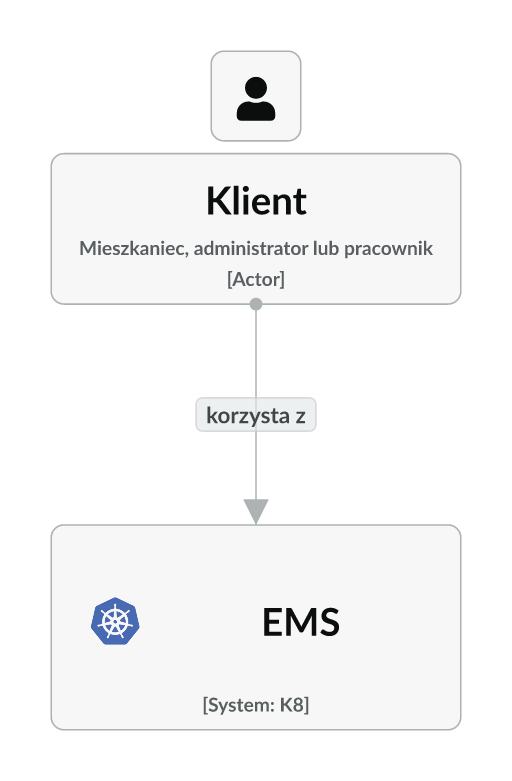
\includegraphics[width=0.5\linewidth]{img/Context_Diagram.png}
    \caption{Kontekst systemu}
    \label{fig:context-diag}
\end{figure}
\subsubsection{Kontener}
Kolejnym poziomem architektury C4 jest poziom kontenerów zaprezentowany poniżej. System został stworzony z użyciem Kubernetesa, tak więc całość jest opisana w klastrze Kubernetesowym z podziałem na poszczególne aplikacje, które zostaną opisane poniżej.
\begin{figure}[H]
    \centering
    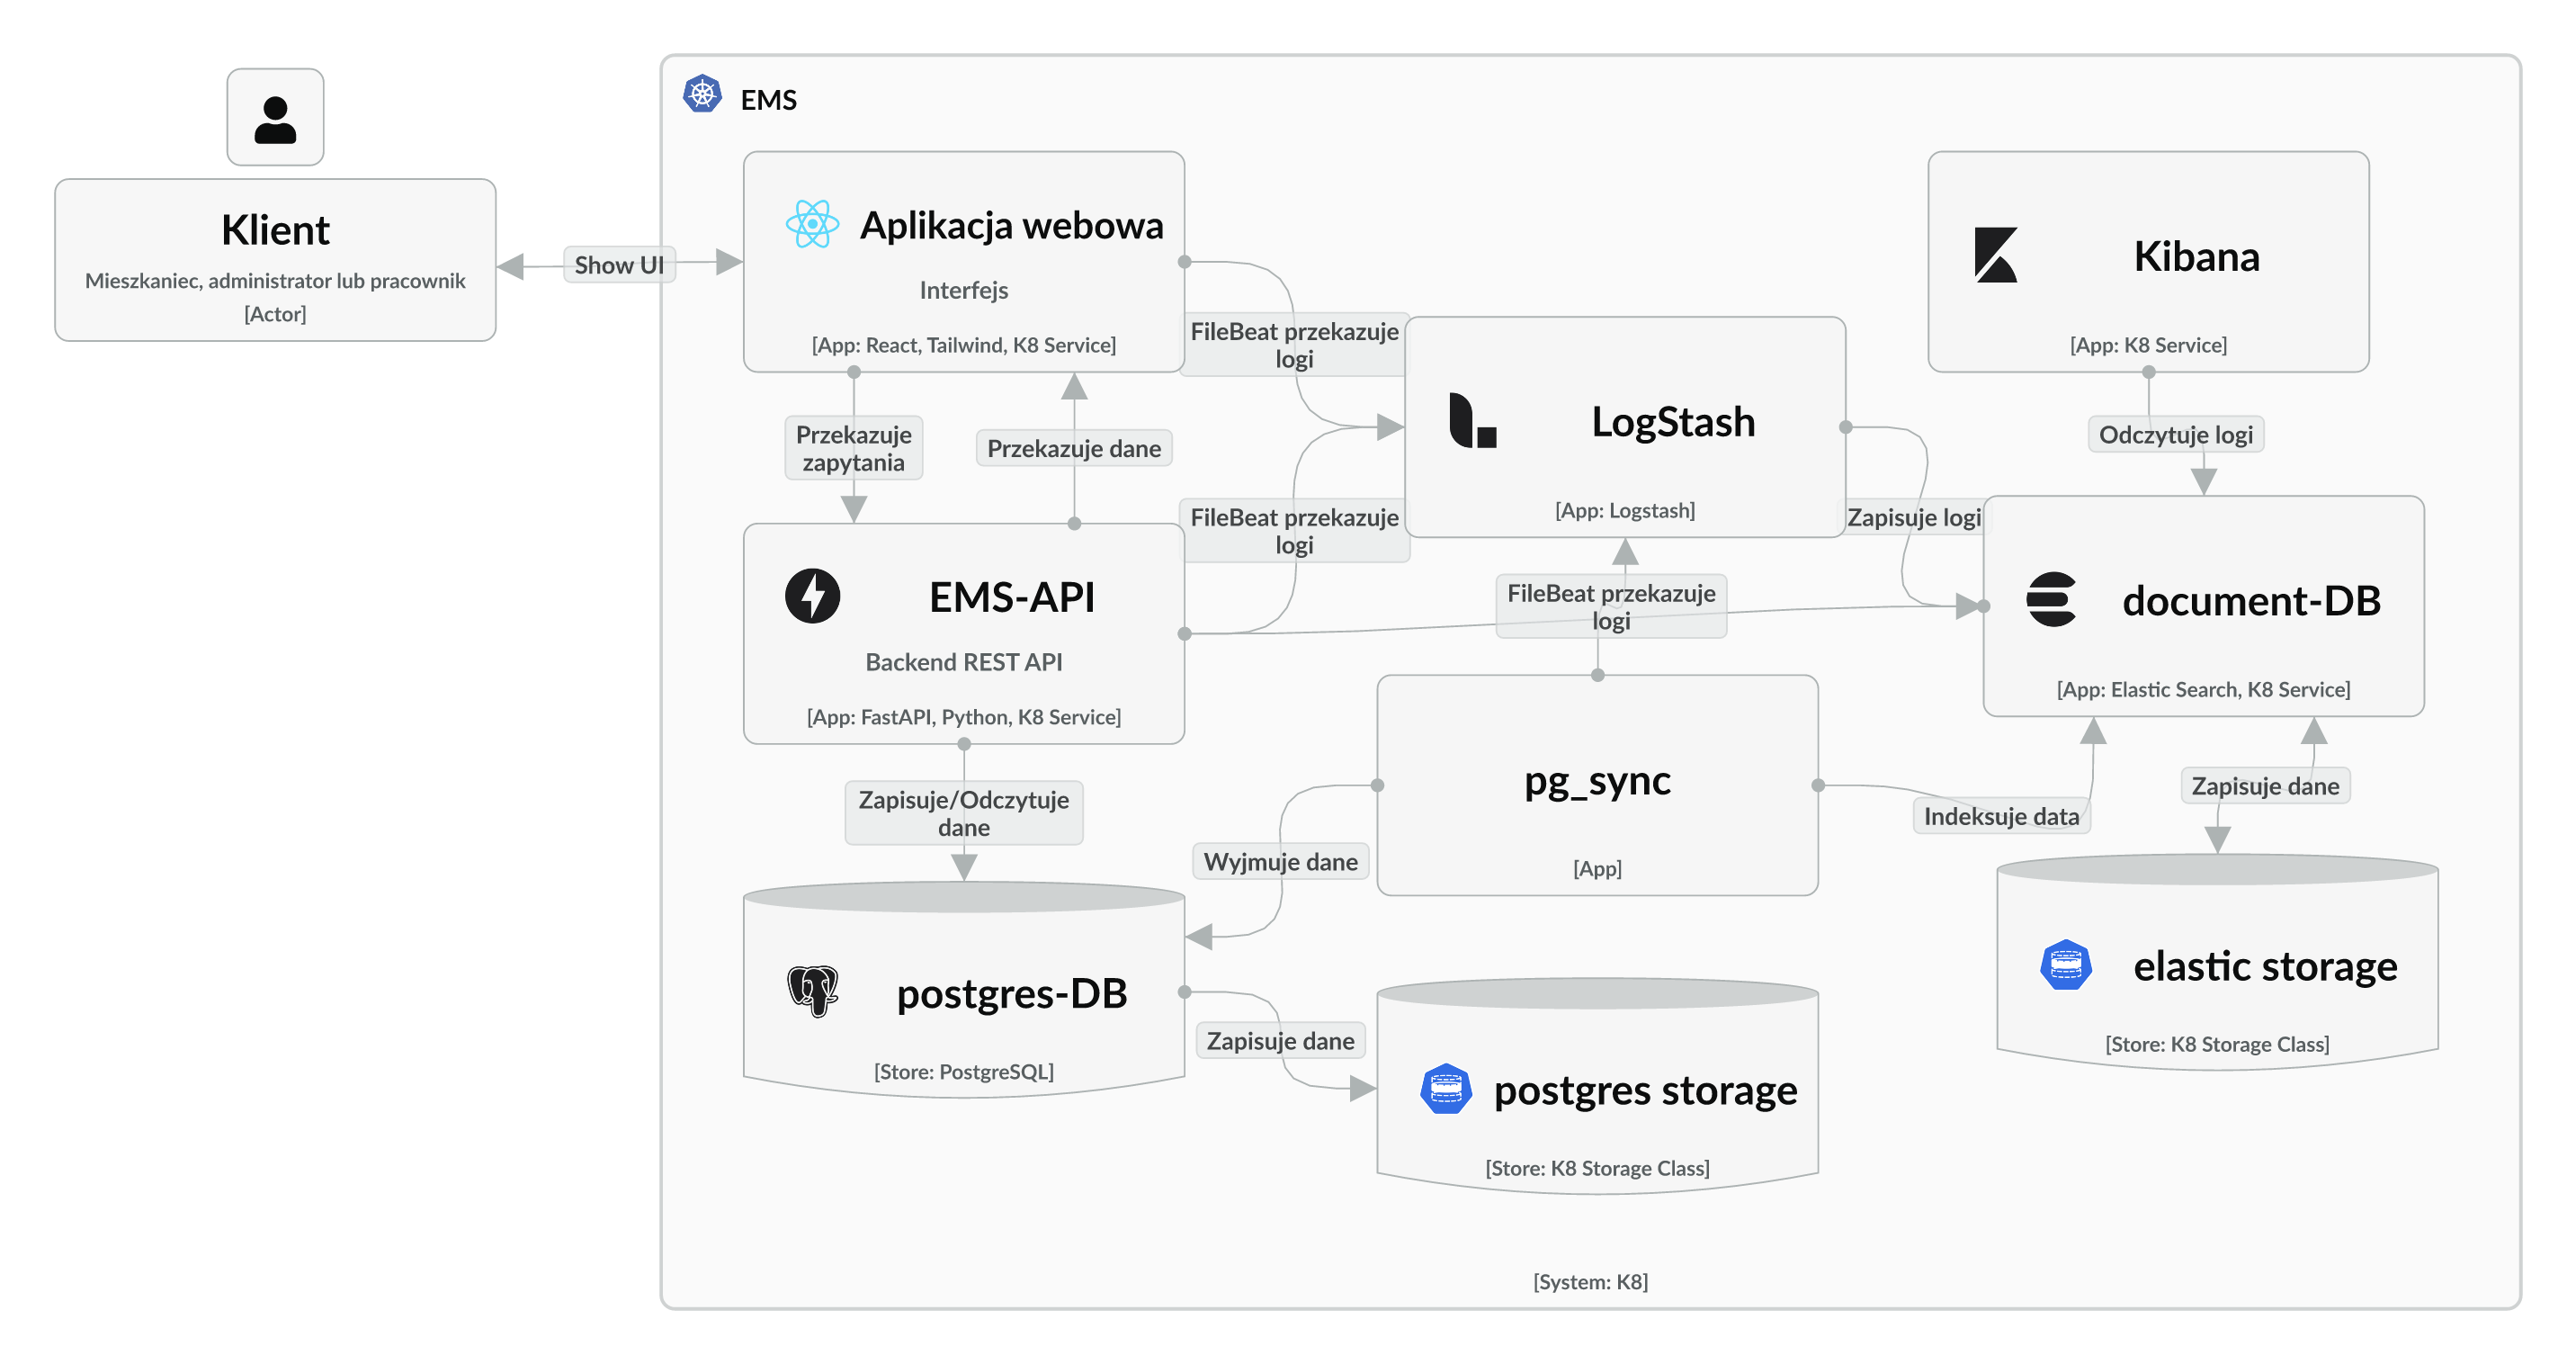
\includegraphics[width=1\linewidth]{img/Container_Diagram.png}
    \caption{Kontenery systemu}
    \label{fig:full-arch}
\end{figure}
Działanie systemu można podzielić na dwie części: część odpowiadającą za realizowanie funkcjonalności, oraz część odpowiadającą za monitorowanie systemu.

\subsubsection{Komponenty odpowiedzialne za realizowanie funkcjonalności}
\begin{itemize}
    \item \textbf{Aplikacja webowa} - jest to deployment Kubernetesowy znajdujący się w Kubernetesowym serwisie, deployment w Kubernetesie ma na celu zarządzanie między innymi na podstawie jakiego obrazu będą uruchamiane pody, oraz ich aktualną ilość kopii. Serwis jest abstrakcją sieciową mającą na celu umożliwienie komunikacji między podami za pomocą ich nazw. Aplikacja napisana została w TypeScript z użyciem React oraz Tailwind. Służy ona do wyświetlania interfejsu użytkownikowi. Interfejs jest dynamicznie renderowany u klienta (CSR). W tym module nie znajduje się żadna logika biznesowa, jest to tylko i wyłącznie warstwa reprezentacyjna komunikująca się z EMS-API.
    \item \textbf{EMS-API} - nazwa pochodzi od nazwy systemu EMS - System do zarządzania osiedlami. Jest to również Kubernetes'owy deployment w Kubernetes'owym serwisie. Jest to aplikacja napisana w Pythonie z użyciem FastApi wystawiający REST-API, z którego korzysta interfejs użytkownika. Moduł ten realizuje logikę biznesową. Komunikuje się on również z dwiema bazami danych: Postgres-DB oraz document-DB. Poniżej przedstawiono schemat reprezentujący znajdujące się w nim komponenty:
    \begin{figure}[H]
        \centering
        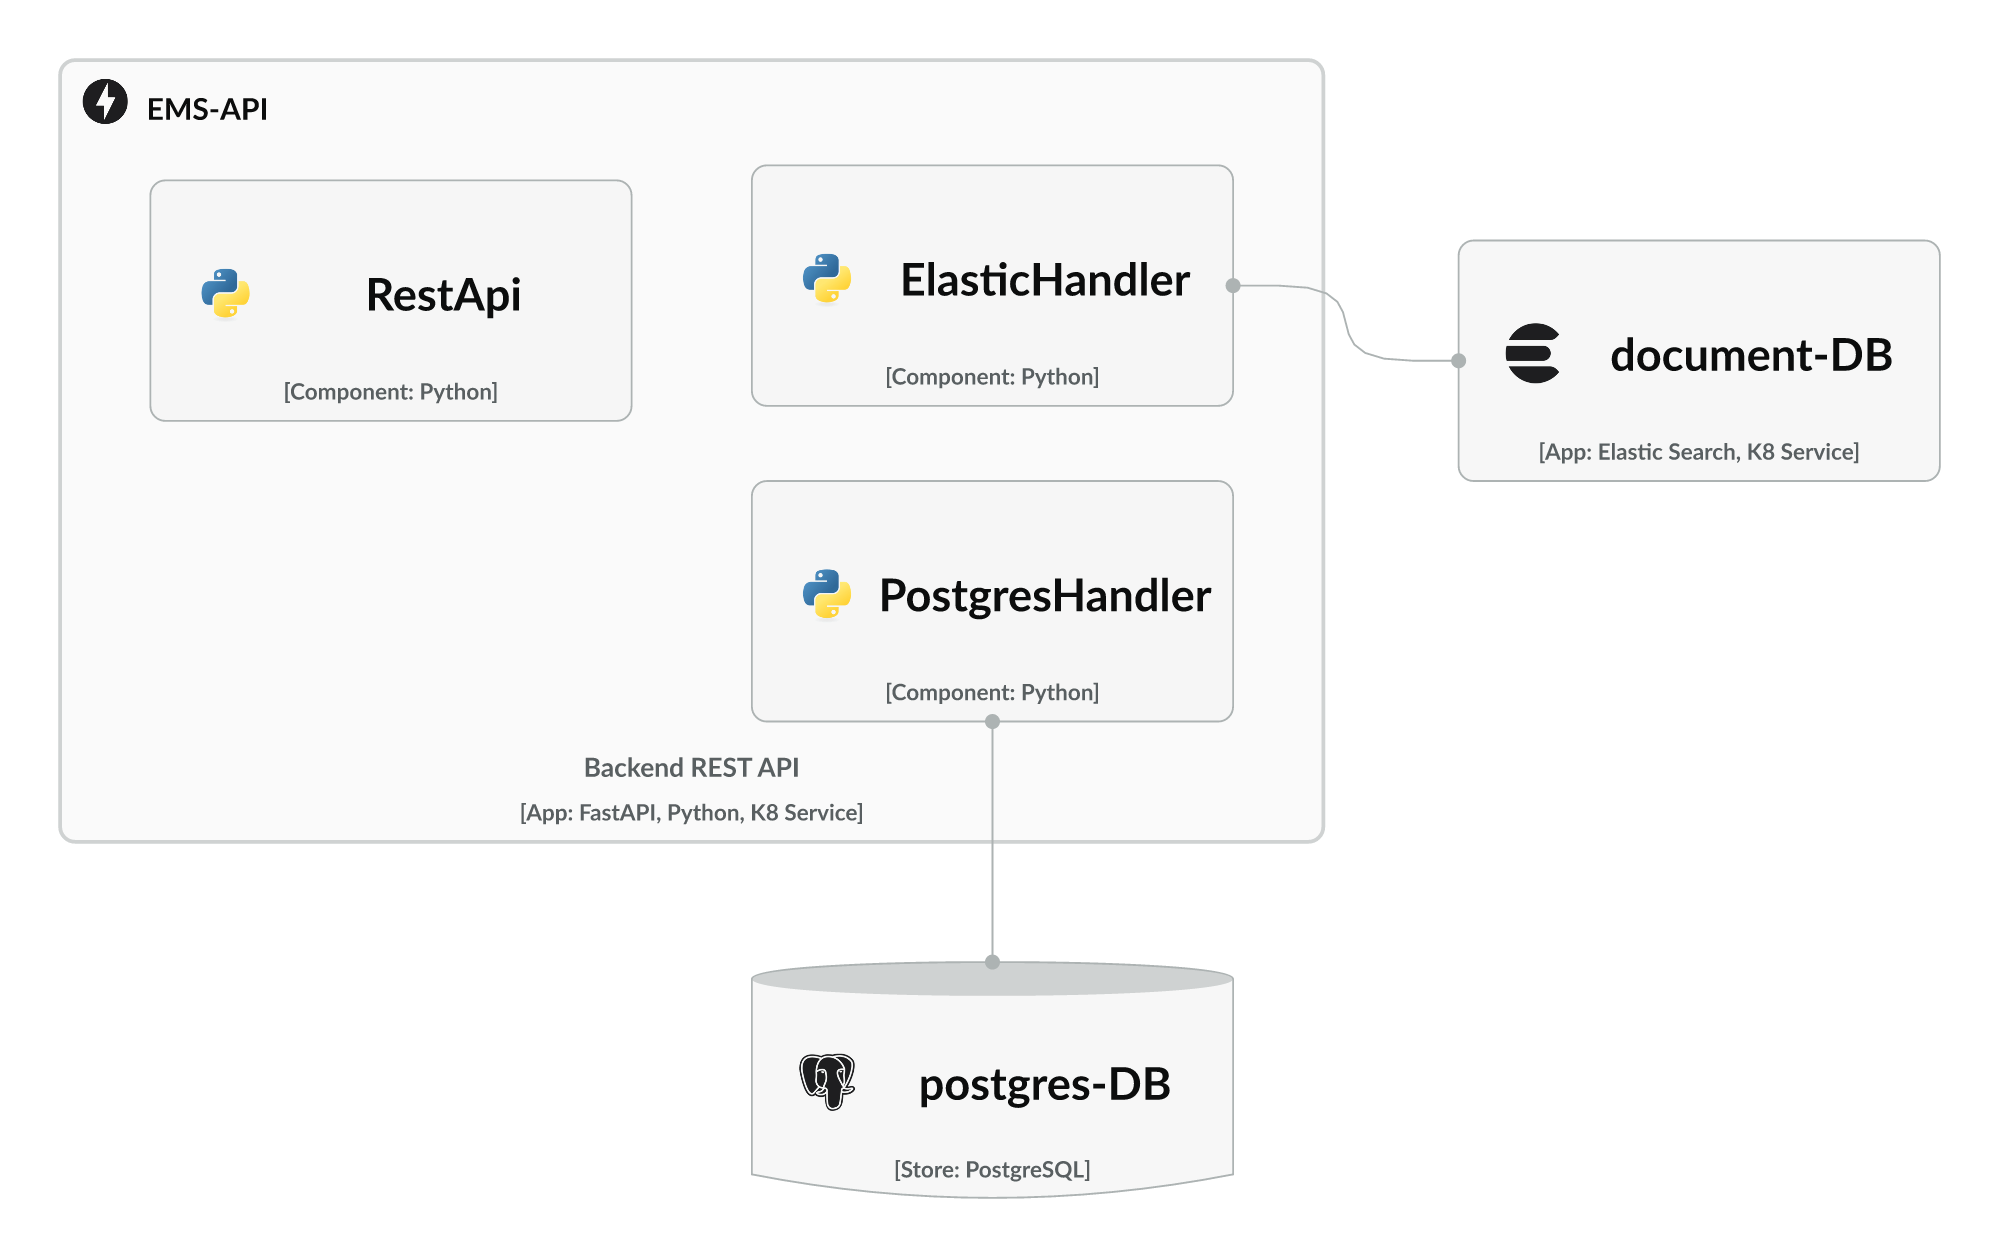
\includegraphics[width=0.75\linewidth]{img/EMS-API Component Diagram (Current).png}
        \caption{Diagram komponentów EMS-API}
        \label{fig:ems-api-components}
    \end{figure}
    \item \textbf{postgres-DB} - Baza relacyjna Postgres, w której zdefiniowane są relacje niezbędne do działania systemu. Jest to również Kubernetes'owy deployment w Kubernetes'owym serwisie.
    \item \textbf{postrges-storage} - Kubernetes'owy storage jest miejscem gdzie Postgres zapisuje dane, jest to niezbędny element, bez którego baza danych nie miała by miejsca na stabilne przetrzymywanie danych, używanie takiej abstrakcji umożliwia również relatywnie niskokosztową zmianę na inny typ storage-u.
    \item \textbf{document-DB} - Jest to baza NoSQL Elasticsearch w tym kontekście wykorzystywana do indeksowania pojedynczych elementów jak i do wyszukiwania elementów na podstawie ich fragmentów.
    \item \textbf{pg\_sync} - Jest to moduł open-source'owy służący do synchronizacji bazy relacyjnej - Postgres, oraz bazy noSQL - Elasticsearch. Moduł ten jest niezbędny ponieważ indeksuje on wybrane elementy w bazie dokumentowej, takimi przykładowymi elementami są np. treści postów. Dzięki temu wyszukiwanie postów na podstawie tekstu wpisanego przez użytkownika jest bardziej optymalne. Takie rozwiązanie odciąża również bazę Postgres - ponieważ wyszukiwanie na podstawie fragmentu tekstu nie jest w niej wykonywane. Moduł ten składa się z 2 elementów: aplikacji w języku Python oraz bazy Redis używanej jako kolejki, co zostało zobrazowane na poniższym diagramie:
    \begin{figure}[H]
        \centering
        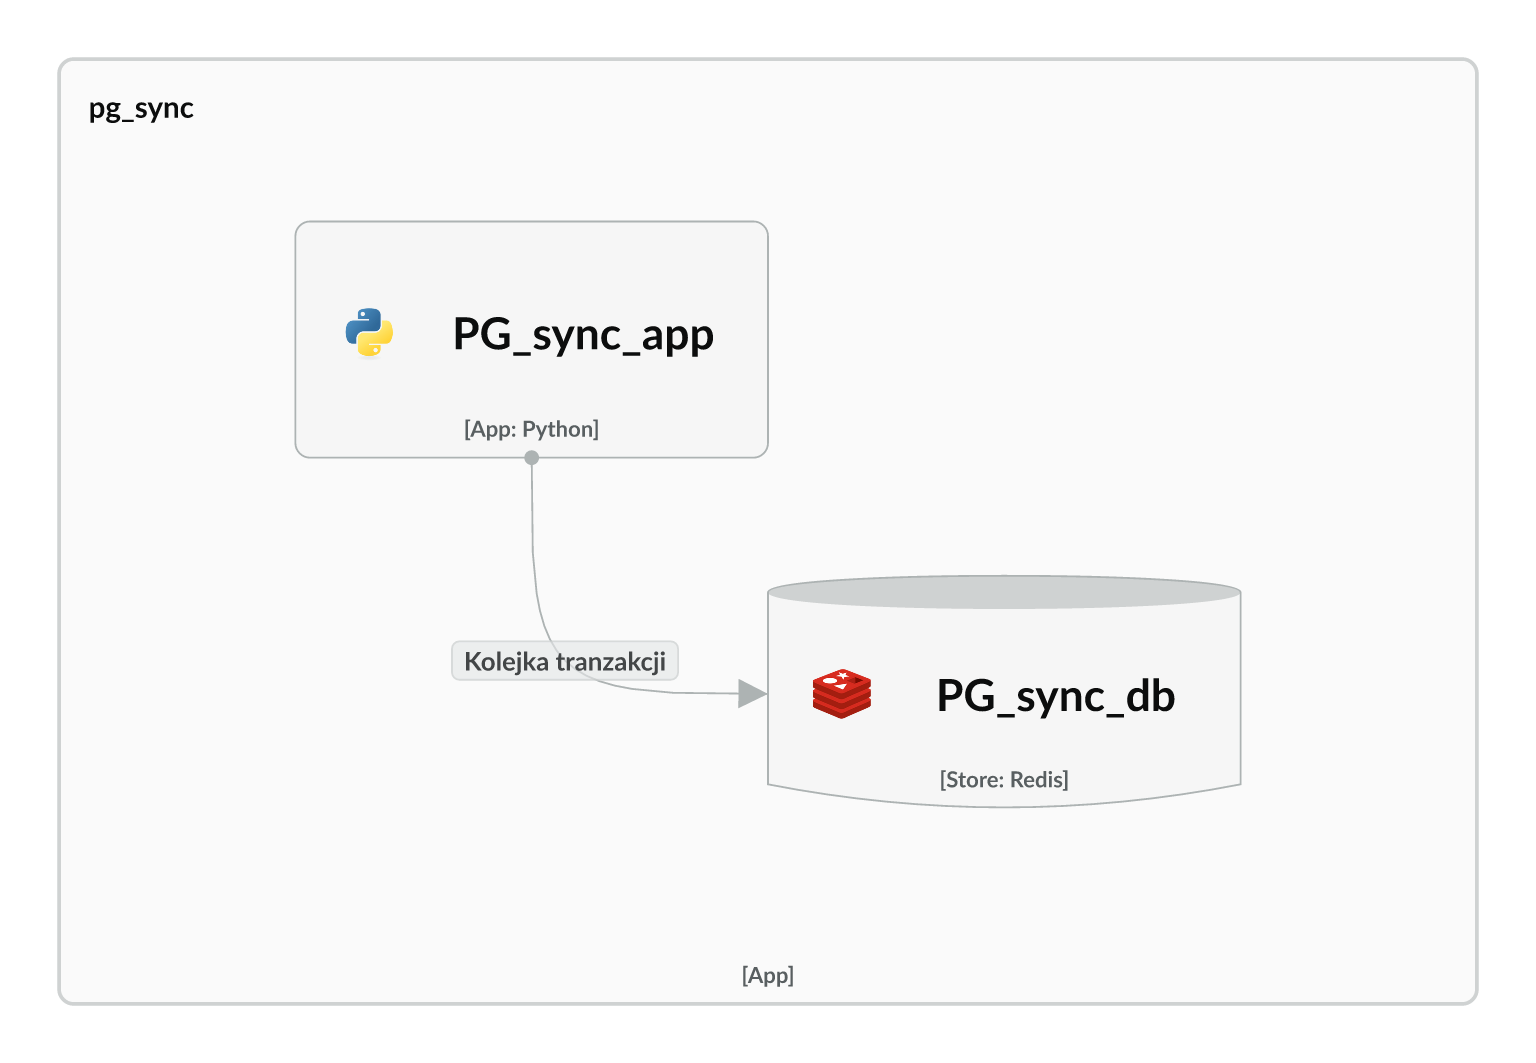
\includegraphics[width=0.75\linewidth]{img/pg_sync Component Diagram (Current).png}
        \caption{Diagram komponentów pg\_sync}
        \label{fig:pg_sync}
    \end{figure}
\end{itemize}
\subsubsection{Przepływ działania systemu  - perspektywa realizacji funkcjonalności}
W celu lepszej wizualizacji działania systemu, poniżej został dodany diagram przykładowego przepływu działania systemu, pokazujący proces dodania ogłoszenia przez użytkownika. Proces pokazuje tylko część systemu odpowiedzialną za działanie funkcjonalności.

\begin{figure}[H]
    \centering
    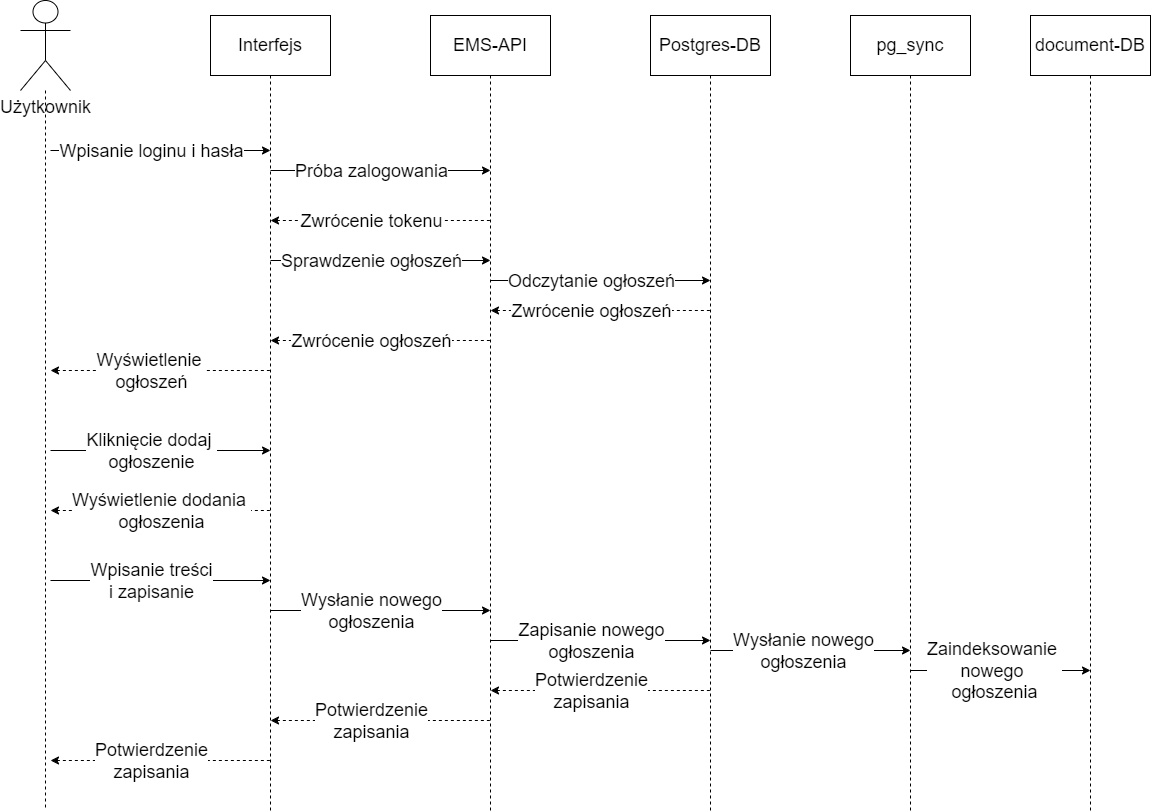
\includegraphics[width=1\linewidth]{img/sequence_diag_add_post.png}
    \caption{Diagram sekwencji dodania ogłoszenia}
    \label{fig:add_post_seq}
\end{figure}
\subsubsection{Komponenty odpowiedzialne za monitorowanie systemu}
\begin{itemize}
    \item \textbf{FileBeat} - Lekki open source'owy moduł stworzony przez firmę Elastic, służący do agregacji i przesyłania odnalezionych plików do skonfigurowanego miejsca, w tym przypadku jest to LogStash. Tak więc jest to komponent odnajdujący automatycznie logi z dodanych serwisów i przekazujący je do LogStash'a.
    \item \textbf{LogStash} - Open source'owe rozwiązanie stworzone przez firmę Elastic, służący do przyjmowania, przetwarzania oraz przekazywania logów do Elasticsearch.
    \item \textbf{document-DB} - Open source'owa baza NoSQL Elasticsearch firmy Elastic, w tym kontekście wykorzystywana jako miejsce zapisu i indeksowania logów.
    \item \textbf{Kibana} - Open source'owe rozwiązanie firmy Elastic stworzone w celu wizualizacji danych znajdujących się w tym przypadku w Elasticsearch, posiada również między innymi możliwość tworzenia dashboard'ów zwiększających potencjał wizualizacji danych, tutaj - logów.
\end{itemize}


\subsection{Decyzje architektoniczne}
\subsubsection{Sposób konteneryzacji, dlaczego Kubernetes?}

Pod uwagę zostało wziętych wiele możliwości konteneryzacji systemów, takich jak:
\begin{itemize}
    \item \textbf{Docker Compose} - Rozwiązanie to umożliwia uruchamianie aplikacji złożonych z wielu kontenerów Docker'owych, nie ma ono wbudowanych wielu możliwości dostępnych w Kubernetes'ie, takich jak równoważenie obciążenia (ang: load balancing). Jest dobre do lokalnego testowania aplikacji, lub wdrażania małych rozwiązań.
    \item \textbf{Docker swarm} - Jest to rozwiązanie wbudowane w silnik Docker'a umożliwiające zarządzanie tworzonymi kontenerami i dostarczające podstawowe funkcjonalności przydatne przy wdrożeniu, takie jak równoważenie obciążenia. Jest ono o wiele mniej popularne od Kubernetes'a i posiada o wiele mniejsze wsparcie. Na podstawie pracy \cite{KubernetesVSDockerSwarm} można wywnioskować, że Kubernetes jest bardziej skomplikowanym narzędziem, posiadającym więcej funkcjonalności, podczas gdy Docker swarm jest rozwiązaniem prostszym i jednocześnie bardziej optymalnym.
    \item \textbf{Podman} - Jest to dobre rozwiązanie do zarządzania pojedynczymi podami na jednej maszynie, nie jest ono dobre do wdrażania dużych aplikacji.
\end{itemize}
Wszystkie te rozwiązania mają swoje plusy i minusy, i po dokładnej ich analizie został wybrany Kubernetes, jako rozwiązanie dostarczające najwięcej możliwości rozwoju, skalowalności i oferujące największe wsparcie społeczności informatycznej.
\subsubsection{Technologia monitorowania działania systemu}
Monitorowanie działania danego systemu jest niezbędnym aspektem, który należy rozważyć, przy prostych aplikacjach skonteneryzowanych na bazie Dockera/Docker-compose często wystarczającym może być obserwowanie logów poszczególnych kontenerów. 

W Kubernetes'ie problem jednak jest większy ze względu na, między innymi, liczbę replik danych aplikacji. Dobrym przykładem jest EMS-API, jest to aplikacja mająca 3 repliki, należy więc wziąć pod uwagę, że w sytuacji wystąpienia błędu, osoba nadzorująca działanie systemu powinna zalogować się na serwer, a następnie wykonać kontrolę  kolejnych logów w każdym podzie, co nie jest ani wygodne ani optymalne.

Często spotykanym rozwiązaniem jest dodatkowy system do monitorowania działania aplikacji, wiele osób korzysta w tym przypadku  z tzw. "ELK stack", będącego połączeniem rozwiązań open-source'owych dostarczonych przez firmę Elastic, w celu monitorowania np. logów. Wymienione rozwiązanie zostało wykorzystane  w projektowanych systemie, z uwagi  na jego popularność i wsparcie społeczeństwa programistycznego. Mając na względzie rozwój aplikacji, jest ono bardzo wygodne, ponieważ dodanie kolejnego elementu systemu nie wymaga praktycznie żadnego nakładu pracy z perspektywy systemu monitoringu, aby ten element również był monitorowany.
\subsubsection{Dobór typu bazy danych}
Do realizacji projektu, będącego celem niniejszej pracy,  wymagana jest baza relacyjna, rynek informatyczny oferuje szeroki wybór dostępnych baz tego rodzaju. Na podstawie analizy artykułu \cite{fi16100382} możemy wywnioskować, że baza Postgres jest o wiele wydajniejsza od bazy MySQL z perspektywy odczytu danych z bazy jak i ich zapisu. Baza Postgres jest odpowiednią bazą do realizacji tego projektu. Aby odciążyć tę bazę można również zutylizować bazę Elasticsearch i indeksować w niej wybrane elemenenty z bazy relacyjnej.
\subsubsection{Sposób synchronizacji Postgres'a z Elasticsearch}
Aby móc użyć 2 baz,  potrzebny jest sposób ich niezawodnej synchronizacji, na rynk dostępnych jest wiele takich  rozwiązań, np: Logstash JDBC input plugin proponowany przez Elastic jako rozwiązanie do synchronizacji bazy Postgres oraz Elasticsearch. Po przeanalizowaniu tego rozwiązania zostało ono odrzucone ze względu na skomplikowaną konfigurację. Rozwiązaniem, które ostatecznie wybranno,  jest pg\_sync open source,  umożliwiające synchronizację bazy Postgres z bazą elastic przy użyciu minimalnej konfiguracji. Pg\_sync złożony jest z aplikacji w Pythonie i kolejki z użyciem Redis'a, tak więc jest to rozwiązanie wygodne do skonteneryzowania, co jest kolejnym atutem.
\subsubsection{Sposób komunikacji z bazami danych}
Istnieje wiele sposobów utworzenia tabel w bazie relacyjnej i komunikacji z nią z perspektywy Pythona. Jedną z możliwości stanowi pisanie plików w SQL, mające na celu tworzenie odpowiednich tabel i funkcji ułatwiających komunikację, ale istnieją też inne dobre rozwiązania. Jednym z takich rozwiązań jest użycie ORM-u: mapowanie obiektowo-relacyjne, polegające na odwzorowaniu relacji z bazy w sposób obiektowy w kodzie. Aby to zrealizować można skorzystać z Pythonowej paczki SQLAlchemy, dzięki czemu nie istnieją pliki w sql tylko i wyłącznie w Pythonie, a tym samym istnieje mniej rozproszonych źródeł oprogramowania, co wspiera zarządzanie wersją i zmniejsza potencjał popełnienia błędów. Dzięki użyciu ORM-a jesteśmy również w stanie napisać testy jednostkowe do metod wykonywanych na bazie. Jednocześnie, zmiana typu bazy z perspektywy kodu aplikacji jest wtedy bardzo prosta - zmieniamy typ silnika ORM-u. Należy rozważyć również  negatywne aspekty tego podejścia, omówione w artykule \cite{ImpactOfORM}, na podstawie którego można wywnioskować, że ORM ma duży wpływ na wydajność zapytań kierowanych do bazy, ale jednocześnie daje on dużą swobodę programistom implementującym użycie bazy z użyciem ORM-a zamiast zapytań SQL.